%%「論文」,「レター」,「レター(C分冊)」,「技術研究報告」などのテンプレート
%% v3.3 [2020/06/02]
%% 1. 「論文」
\documentclass[technicalreport]{ieicej}
%\documentclass[invited]{ieicej}% 招待論文
%\documentclass[survey]{ieicej}% サーベイ論文
%\documentclass[comment]{ieicej}% 解説論文
%\usepackage[dvips]{graphicx}
%\usepackage[dvipdfmx]{graphicx,xcolor}
\usepackage[fleqn]{amsmath}
\usepackage{newtxtext}% 英数字フォントの設定を変更しないでください
\usepackage[varg]{newtxmath}% % 英数字フォントの設定を変更しないでください
\usepackage{latexsym}
%\usepackage{amssymb}
\usepackage[dvipdfmx]{graphicx}
\graphicspath{ {./img/} }

\setcounter{page}{1}

\field{}
\jtitle{Beyond 5G高周波通信の空間分解能を 向上するための誘電体導波路の研究}
\etitle{Research on Dielectric Waveguides for Enhancing Spatial Resolution in Beyond 5G High Frequency Communications}
\authorlist{%
 \authorentry[mitani-reishi116@g.ecc.u-tokyo.ac.jp]{三谷怜司}{Reishi Mitani}{東京大学 〒113-0033 東京都文京区本郷 7-3-1}\MembershipNumber{}
 \authorentry[nakao@nakao-lab.org]{中尾彰宏}{Akihiro Nakao}{東京大学 〒113-0033 東京都文京区本郷 7-3-1}\MembershipNumber{}
 %\authorentry{和文著者名}{英文著者名}{所属ラベル}\MembershipNumber{}
 %\authorentry[メールアドレス]{和文著者名}{英文著者名}{所属ラベル}\MembershipNumber{}
 %\authorentry{和文著者名}{英文著者名}{所属ラベル}[現在の所属ラベル]\MembershipNumber{}
}
\affiliate[]{東京大学 〒113-0033 東京都文京区本郷 7-3-1}{The University of Tokyo, Graduate School of Interdisciplinary Information Studies 7-3-1, Hongo, Bunkyo-ku, Tokyo, 113-0033 Japan}
%\affiliate[所属ラベル]{和文所属}{英文所属}
%\paffiliate[]{}
%\paffiliate[現在の所属ラベル]{和文所属}
\jalcdoi{???????????}% ← このままにしておいてください

\begin{document}
\begin{abstract}
  5G・Beyond5Gで普及が期待されている高周波数の通信では
  帯域を広く利用することで大容量の通信が可能となる一方
  電波伝播の直進性や急激な減衰から利活用の困難さが指摘されている。
  我々は、ミリ波などの高周波数を利用する通信において、直進性や減衰性を逆に利用し、
  高空間分解能の通信に利活用することを考えている。
  一般に、ミリ波ではアレイアンテナを利用するビームフォーミングにより電波伝播の範囲を
  限定することが可能であるが、コストが高いなどの課題がある。
  本研究では、低コストでビームを絞るための誘電体導波路を用いたミリ波アンテナを設計・
  製作することを提案し
  シミュレーション評価によりその有用性を示す。
\end{abstract}
\begin{keyword}
%和文キーワード 4〜5語
Beyond5G
\end{keyword}
\begin{eabstract}
%英文アブストラクト 100 words
High-frequency communications,
which are expected to be widely used in 5G and Beyond5G,
enable high-capacity communications by using a wide bandwidth.
However, the linearity of radio wave propagation and rapid attenuation
have made it difficult to utilize high-frequency communications.
In this paper, we consider the use of millimeter waves and
other high-frequency communications for high-spatial-resolution communications
by taking advantage of their linearity and attenuation.
Generally, it is possible to limit the range of radio propagation by
beamforming using array antennas in millimeter-wave communications,
but there is a problem of high cost.
In this study,
we propose to design and fabricate a millimeter-wave antenna using
dielectric waveguides to narrow the beam at low cost,
and demonstrate its usefulness through simulation evaluation.
\end{eabstract}
\begin{ekeyword}
%英文キーワード
Beyond5G
\end{ekeyword}
\maketitle

\section{はじめに}

第5世代移動通信システム(5G)の商用サービスが2020年3月に開始され、
移動通信システムとしては初めて、28GHz帯を利用した広帯域高速通信が実用化された。
28GHz以上のミリ波の帯域の利用は今後拡大されることが予想される。

5G・Beyond5Gで普及が期待されている高周波数の通信では、
帯域を広く利用することで大容量の通信が可能となる一方、
電波伝播の直進性や急激な減衰から利活用の困難さが指摘されている。
また、ミリ波は高分解能があるにもかかわらず、
それを生かしたセキュリティを確立する方法が難しい。
ここでいうセキュリティというのは以下のことを示す。

\begin{itemize}
  \item デバイスが多い環境においては、それぞれのデバイスへの電波の割り当てが困難となる
  \item 渡すべきでない情報を他のデバイスに渡してしまうことがありえる
\end{itemize}

セキュリティを向上する既存の方法では以下の障害が存在する。
一つ目はミリ波専用の機器はハード、ソフトともに開発コストがかかるうえ、
ミリ波は波長が短く、より精密なエンジニアリングが必要となることである。
MIMOなどを実装し、ビームフォーミングを可能にすることでセキュリティ
を向上することも可能だが、これも開発と実装、そしてチューニングのコストがかかる。
二つ目はリードタイムが長いことで、ホーンアンテナなどの機器は納品までに時間がかかる。
これもより精密なエンジニアリングが必要となることに起因する。
3つ目にインフラが柔軟でないことがあげられる。
ホーンアンテナなどの機器は一度配置してしまうと場所を変えにくいため、
設計などに気を付けなければならない。

本論文の構成は次の通りである.次章では,本研究
に関連する技術について述べる.第3章,第4章では,
システム概要を示した提案手法と実際の実装について
まとめる.第5章にて,各ケースにおけるスループット
やFPSの評価を行い,第6章で今後の展望について考察
する.最終章にて本論文をまとめる.

\section{関連技術}

\subsection{既存の伝送媒体}

ミリ波の伝送媒体には主に以下が利用される。
\begin{itemize}
  \item 導波管
  \item 同軸ケーブル
  \item 誘電体導波路
\end{itemize}

導波管は誘電体または空気の周囲を導体で囲んだ断面形状をもち、衛星地球局で利用される。
ただ容易に曲げることができず、重いという制約がある。
同軸ケーブルは中心導体と外部導体が同心円状に配置された断面形状をもち、
おもにマイクロ波以下の周波数帯で利用される。
こちらは高周波数帯での損失が導波管よりも高いという制約があります。

誘電体導波路は棒状の誘電体の周囲を異なる誘電率を有する誘電体で囲んだ構造を持ち、
高周波数帯電波の伝送のために使われることが多い
導波管と同軸ケーブルを足して2で割ったような特徴を持ち、
損失は発生するが、同軸ケーブルよりは低い上、軽くて柔軟に曲げることができる。

\begin{figure}
  \begin{center}    
    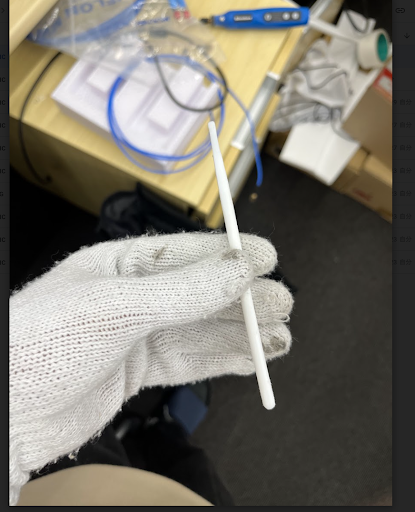
\includegraphics[clip, keepaspectratio, width=0.5\linewidth]{img/waveguide.png}
    \caption{誘電体導波路}
    \label{fig:metal_waveguide}
  \end{center}
\end{figure}

\section{提案手法}

\subsection{}

\section{シミュレーション}

\section{結果と評価}

\section{今後の展望}

\section{結論}



\ack %% 謝辞
本研究の一部は株式会社NTT Docomoの助成を受けたものです.
共同での実験環境・機材等のご支援を頂き,誠に感謝致します.

%\bibliographystyle{sieicej}
%\bibliography{myrefs}
\begin{thebibliography}{99}% 文献数が10未満の時 {9}
\bibitem{}
\end{thebibliography}

\appendix
\section{}

\begin{biography}
\profile{}{}{}
%\profile{会員種別}{名前}{紹介文}% 顔写真あり
%\profile*{会員種別}{名前}{紹介文}% 顔写真なし
\end{biography}

\end{document}



%% 2. 「レター」
\documentclass[letter]{ieicej}
%\usepackage[dvips]{graphicx}
%\usepackage[dvipdfmx]{graphicx,xcolor}
\usepackage[fleqn]{amsmath}
\usepackage{newtxtext}% 英数字フォントの設定を変更しないでください
\usepackage[varg]{newtxmath}% % 英数字フォントの設定を変更しないでください
\usepackage{latexsym}
%\usepackage{amssymb}

\setcounter{page}{1}

\typeofletter{研究速報}
%\typeofletter{紙上討論}
%\typeofletter{問題提起}
%\typeofletter{ショートノート}
\field{}
\jtitle{}
\etitle{}
\authorlist{%
 \authorentry{}{}{}{}\MembershipNumber{}
 %\authorentry{和文著者名}{英文著者名}{会員種別}{所属ラベル}\MembershipNumber{}
 %\authorentry{和文著者名}{英文著者名}{会員種別}{所属ラベル}[現在の所属ラベル]\MembershipNumber{}
}
\affiliate[]{}{}
%\affiliate[所属ラベル]{和文所属}{英文所属}
%\paffiliate[]{}
%\paffiliate[現在の所属ラベル]{和文所属}
\jalcdoi{???????????}% ← このままにしておいてください

\begin{document}
\maketitle
\begin{abstract}
%和文あらまし 120字以内
\end{abstract}
\begin{keyword}
%和文キーワード 4〜5語
\end{keyword}
\begin{eabstract}
%英文アブストラクト 50 words
\end{eabstract}
\begin{ekeyword}
%英文キーワード
\end{ekeyword}

\section{まえがき}


\ack %% 謝辞

%\bibliographystyle{sieicej}
%\bibliography{myrefs}
\begin{thebibliography}{99}% 文献数が10未満の時 {9}
\bibitem{}
\end{thebibliography}

\appendix
\section{}

\end{document}


%% 3. 「レター(C分冊)」
\documentclass[electronicsletter]{ieicej}
%\usepackage[dvips]{graphicx}
%\usepackage[dvipdfmx]{graphicx,xcolor}
\usepackage[fleqn]{amsmath}
\usepackage{newtxtext}% 英数字フォントの設定を変更しないでください
\usepackage[varg]{newtxmath}% % 英数字フォントの設定を変更しないでください
\usepackage{latexsym}
%\usepackage{amssymb}

\setcounter{page}{1}

\field{}
\jtitle{}
\etitle{}
\authorlist{%
 \authorentry{}{}{}{}\MembershipNumber{}
 %\authorentry{和文著者名}{英文著者名}{会員種別}{所属ラベル}\MembershipNumber{}
 %\authorentry{和文著者名}{英文著者名}{会員種別}{所属ラベル}[現在の所属ラベル]\MembershipNumber{}
}
\affiliate[]{}{}
%\affiliate[所属ラベル]{和文所属}{英文所属}
%\paffiliate[]{}
%\paffiliate[現在の所属ラベル]{和文所属}
\jalcdoi{???????????}% ← このままにしておいてください

\begin{document}
\begin{abstract}
%和文あらまし 120字以内
\end{abstract}
\begin{keyword}
%和文キーワード 4〜5語
\end{keyword}
\begin{eabstract}
%英文アブストラクト 50 words
\end{eabstract}
\begin{ekeyword}
%英文キーワード
\end{ekeyword}
\maketitle

\section{まえがき}


\ack %% 謝辞

%\bibliographystyle{sieicej}
%\bibliography{myrefs}
\begin{thebibliography}{99}% 文献数が 10 未満の時 {9}
\bibitem{}
\end{thebibliography}

\appendix
\section{}

\end{document}



%% 4. 「技術研究報告」
\documentclass[technicalreport]{ieicej}
%\usepackage[dvips]{graphicx}
%\usepackage[dvipdfmx]{graphicx,xcolor}
\usepackage[fleqn]{amsmath}
\usepackage{newtxtext}% 英数字フォントの設定を変更しないでください
\usepackage[varg]{newtxmath}% % 英数字フォントの設定を変更しないでください
\usepackage{latexsym}
%\usepackage{amssymb}

\jtitle{}
\jsubtitle{}
\etitle{}
\esubtitle{}
\authorlist{%
 \authorentry[]{}{}{}
% \authorentry[メールアドレス]{和文著者名}{英文著者名}{所属ラベル}
}
\affiliate[]{}{}
%\affiliate[所属ラベル]{和文勤務先\\ 連絡先住所}{英文勤務先\\ 英文連絡先住所}
\jalcdoi{???????????}% ← このままにしておいてください

\begin{document}
\begin{jabstract}
%和文あらまし
\end{jabstract}
\begin{jkeyword}
%和文キーワード
\end{jkeyword}
\begin{eabstract}
%英文アブストラクト
\end{eabstract}
\begin{ekeyword}
%英文キーワード
\end{ekeyword}
\maketitle

\section{はじめに}


%\bibliographystyle{sieicej}
%\bibliography{myrefs}
\begin{thebibliography}{99}% 文献数が10未満の時 {9}
\bibitem{}
\end{thebibliography}

\end{document}
